% Options for packages loaded elsewhere
\PassOptionsToPackage{unicode}{hyperref}
\PassOptionsToPackage{hyphens}{url}
%
\documentclass[
]{article}
\usepackage{amsmath,amssymb}
\usepackage{iftex}
\ifPDFTeX
  \usepackage[T1]{fontenc}
  \usepackage[utf8]{inputenc}
  \usepackage{textcomp} % provide euro and other symbols
\else % if luatex or xetex
  \usepackage{unicode-math} % this also loads fontspec
  \defaultfontfeatures{Scale=MatchLowercase}
  \defaultfontfeatures[\rmfamily]{Ligatures=TeX,Scale=1}
\fi
\usepackage{lmodern}
\ifPDFTeX\else
  % xetex/luatex font selection
\fi
% Use upquote if available, for straight quotes in verbatim environments
\IfFileExists{upquote.sty}{\usepackage{upquote}}{}
\IfFileExists{microtype.sty}{% use microtype if available
  \usepackage[]{microtype}
  \UseMicrotypeSet[protrusion]{basicmath} % disable protrusion for tt fonts
}{}
\makeatletter
\@ifundefined{KOMAClassName}{% if non-KOMA class
  \IfFileExists{parskip.sty}{%
    \usepackage{parskip}
  }{% else
    \setlength{\parindent}{0pt}
    \setlength{\parskip}{6pt plus 2pt minus 1pt}}
}{% if KOMA class
  \KOMAoptions{parskip=half}}
\makeatother
\usepackage{xcolor}
\usepackage[margin=1in]{geometry}
\usepackage{color}
\usepackage{fancyvrb}
\newcommand{\VerbBar}{|}
\newcommand{\VERB}{\Verb[commandchars=\\\{\}]}
\DefineVerbatimEnvironment{Highlighting}{Verbatim}{commandchars=\\\{\}}
% Add ',fontsize=\small' for more characters per line
\usepackage{framed}
\definecolor{shadecolor}{RGB}{248,248,248}
\newenvironment{Shaded}{\begin{snugshade}}{\end{snugshade}}
\newcommand{\AlertTok}[1]{\textcolor[rgb]{0.94,0.16,0.16}{#1}}
\newcommand{\AnnotationTok}[1]{\textcolor[rgb]{0.56,0.35,0.01}{\textbf{\textit{#1}}}}
\newcommand{\AttributeTok}[1]{\textcolor[rgb]{0.13,0.29,0.53}{#1}}
\newcommand{\BaseNTok}[1]{\textcolor[rgb]{0.00,0.00,0.81}{#1}}
\newcommand{\BuiltInTok}[1]{#1}
\newcommand{\CharTok}[1]{\textcolor[rgb]{0.31,0.60,0.02}{#1}}
\newcommand{\CommentTok}[1]{\textcolor[rgb]{0.56,0.35,0.01}{\textit{#1}}}
\newcommand{\CommentVarTok}[1]{\textcolor[rgb]{0.56,0.35,0.01}{\textbf{\textit{#1}}}}
\newcommand{\ConstantTok}[1]{\textcolor[rgb]{0.56,0.35,0.01}{#1}}
\newcommand{\ControlFlowTok}[1]{\textcolor[rgb]{0.13,0.29,0.53}{\textbf{#1}}}
\newcommand{\DataTypeTok}[1]{\textcolor[rgb]{0.13,0.29,0.53}{#1}}
\newcommand{\DecValTok}[1]{\textcolor[rgb]{0.00,0.00,0.81}{#1}}
\newcommand{\DocumentationTok}[1]{\textcolor[rgb]{0.56,0.35,0.01}{\textbf{\textit{#1}}}}
\newcommand{\ErrorTok}[1]{\textcolor[rgb]{0.64,0.00,0.00}{\textbf{#1}}}
\newcommand{\ExtensionTok}[1]{#1}
\newcommand{\FloatTok}[1]{\textcolor[rgb]{0.00,0.00,0.81}{#1}}
\newcommand{\FunctionTok}[1]{\textcolor[rgb]{0.13,0.29,0.53}{\textbf{#1}}}
\newcommand{\ImportTok}[1]{#1}
\newcommand{\InformationTok}[1]{\textcolor[rgb]{0.56,0.35,0.01}{\textbf{\textit{#1}}}}
\newcommand{\KeywordTok}[1]{\textcolor[rgb]{0.13,0.29,0.53}{\textbf{#1}}}
\newcommand{\NormalTok}[1]{#1}
\newcommand{\OperatorTok}[1]{\textcolor[rgb]{0.81,0.36,0.00}{\textbf{#1}}}
\newcommand{\OtherTok}[1]{\textcolor[rgb]{0.56,0.35,0.01}{#1}}
\newcommand{\PreprocessorTok}[1]{\textcolor[rgb]{0.56,0.35,0.01}{\textit{#1}}}
\newcommand{\RegionMarkerTok}[1]{#1}
\newcommand{\SpecialCharTok}[1]{\textcolor[rgb]{0.81,0.36,0.00}{\textbf{#1}}}
\newcommand{\SpecialStringTok}[1]{\textcolor[rgb]{0.31,0.60,0.02}{#1}}
\newcommand{\StringTok}[1]{\textcolor[rgb]{0.31,0.60,0.02}{#1}}
\newcommand{\VariableTok}[1]{\textcolor[rgb]{0.00,0.00,0.00}{#1}}
\newcommand{\VerbatimStringTok}[1]{\textcolor[rgb]{0.31,0.60,0.02}{#1}}
\newcommand{\WarningTok}[1]{\textcolor[rgb]{0.56,0.35,0.01}{\textbf{\textit{#1}}}}
\usepackage{graphicx}
\makeatletter
\def\maxwidth{\ifdim\Gin@nat@width>\linewidth\linewidth\else\Gin@nat@width\fi}
\def\maxheight{\ifdim\Gin@nat@height>\textheight\textheight\else\Gin@nat@height\fi}
\makeatother
% Scale images if necessary, so that they will not overflow the page
% margins by default, and it is still possible to overwrite the defaults
% using explicit options in \includegraphics[width, height, ...]{}
\setkeys{Gin}{width=\maxwidth,height=\maxheight,keepaspectratio}
% Set default figure placement to htbp
\makeatletter
\def\fps@figure{htbp}
\makeatother
\setlength{\emergencystretch}{3em} % prevent overfull lines
\providecommand{\tightlist}{%
  \setlength{\itemsep}{0pt}\setlength{\parskip}{0pt}}
\setcounter{secnumdepth}{-\maxdimen} % remove section numbering
\usepackage{booktabs}
\usepackage{longtable}
\usepackage{array}
\usepackage{multirow}
\usepackage{wrapfig}
\usepackage{float}
\usepackage{colortbl}
\usepackage{pdflscape}
\usepackage{tabu}
\usepackage{threeparttable}
\usepackage{threeparttablex}
\usepackage[normalem]{ulem}
\usepackage{makecell}
\usepackage{xcolor}
\ifLuaTeX
  \usepackage{selnolig}  % disable illegal ligatures
\fi
\usepackage{bookmark}
\IfFileExists{xurl.sty}{\usepackage{xurl}}{} % add URL line breaks if available
\urlstyle{same}
\hypersetup{
  hidelinks,
  pdfcreator={LaTeX via pandoc}}

\author{}
\date{\vspace{-2.5em}}

\begin{document}

\subsection{}\label{section}

\subsection{}\label{section-1}

Entrega B: R - Evaluación de Modelos

Andrés García-Serra Romero Ciencia de Datos

\subsection{}\label{section-2}

Introducción

En este trabajo aplicaremos los conocimientos aprendidos en evaluación
de diferentes tipos de clasificadores de datos en la tarea de predicción
de si un indivíduo ha ganado o no una partida de tres en raya,
utilizando como datos de input la distribución del tablero de la
partida. Para realizar la práctica hemos utilizado el software RStudio,
creando un proyecto del tipo Markdown notebook. Utilizando el paquete
\emph{caret} de \emph{R} entrenaremos cuatro modelos: Un Naive Bayes, un
modelo de Árboles de Decisión, una Red Neuronal, uno de Nearest
Neighbours y finalmente un SVM con kernel lineal. Estos modelos serán
entenados todos usando Cross-Validation y los mismos sets de
entrenamiento y evaluación, divididiendo el set total de datos al 70/30
respectivamente.

Explicaremos en primer lugar cómo hemos llevado a cabo la división del
set global de datos manteniendo la proporción de clases y comprobando
que todos los datos sean correctos. Seguidamente entrenaremos los
modelos, mostrando las métricas de entrenamiento de cada modelo y
evaluaremos los modelos usando el set de evaulación, para lo cual
calcularemos distintas métricas (incluyendo el AUC) para comprobar la
validez de cada uno de los clasificadores según sus curvas ROC.
Finalmente, responderemos las preguntas planteadas en el enunciado de la
tarea.

\subsection{}\label{section-3}

1. Importar Datos

En primer lugar importaremos el fichero \emph{tic-tac-toe.txt} con los
datos en un dataframe, del que cambiaremos los nombres de las columnas
para comprender mejor los datos. Para esto tendremos en cuenta de que se
trata de un tablero 3x3 en el que las posiciones van desde arriba a la
izquierda (\emph{pos1}) hasta debajo a la derecha (\emph{pos9}).
Llamaremos \emph{win} al último elemento de cada fila, que recoge la
victoria o derrota del jugador ``x''. Aquí podemos ver un ejemplo para
entender mejor la distribución de los datos, siendo un ejemplo
aleatorio, no real.

Para el caso real, podemos generar una tabla que recoge las primeras 6
filas de nuestro dataframe ya modificado.

\begin{Shaded}
\begin{Highlighting}[]
\NormalTok{tictac }\OtherTok{\textless{}{-}} \FunctionTok{data.frame}\NormalTok{(}\FunctionTok{read.csv}\NormalTok{(}\StringTok{"tic{-}tac{-}toe.txt"}\NormalTok{))}
\NormalTok{header }\OtherTok{\textless{}{-}} \FunctionTok{c}\NormalTok{(}\StringTok{"pos1"}\NormalTok{,}\StringTok{"pos2"}\NormalTok{,}\StringTok{"pos3"}\NormalTok{,}\StringTok{"pos4"}\NormalTok{,}\StringTok{"pos5"}\NormalTok{,}\StringTok{"pos6"}\NormalTok{,}\StringTok{"pos7"}\NormalTok{,}\StringTok{"pos8"}\NormalTok{,}\StringTok{"pos9"}\NormalTok{,}\StringTok{"win"}\NormalTok{)}
\FunctionTok{colnames}\NormalTok{(tictac) }\OtherTok{\textless{}{-}}\NormalTok{ header}
\FunctionTok{head}\NormalTok{(tictac)}
\end{Highlighting}
\end{Shaded}

\begin{verbatim}
##   pos1 pos2 pos3 pos4 pos5 pos6 pos7 pos8 pos9      win
## 1    x    x    x    x    o    o    o    x    o positive
## 2    x    x    x    x    o    o    o    o    x positive
## 3    x    x    x    x    o    o    o    b    b positive
## 4    x    x    x    x    o    o    b    o    b positive
## 5    x    x    x    x    o    o    b    b    o positive
## 6    x    x    x    x    o    b    o    o    b positive
\end{verbatim}

Como último paso dentro del input de datos, analizamos en busca de
valores vacíos, NaNs o valores que no sean los deseados, es decir:
``x'', ``o'' o ``b'' entre los componentes de posición y ``positive'' o
``negative'' en el último elemento de cada fila.

\begin{Shaded}
\begin{Highlighting}[]
\FunctionTok{any}\NormalTok{(}\FunctionTok{is.na}\NormalTok{(tictac))}
\NormalTok{values }\OtherTok{\textless{}{-}} \FunctionTok{c}\NormalTok{(}\StringTok{"x"}\NormalTok{, }\StringTok{"o"}\NormalTok{, }\StringTok{"b"}\NormalTok{,}\StringTok{"positive"}\NormalTok{, }\StringTok{"negative"}\NormalTok{)}
\FunctionTok{any}\NormalTok{(}\SpecialCharTok{!}\FunctionTok{as.matrix}\NormalTok{(tictac[, }\DecValTok{1}\SpecialCharTok{:}\DecValTok{9}\NormalTok{]) }\SpecialCharTok{\%in\%}\NormalTok{ values[}\DecValTok{1}\SpecialCharTok{:}\DecValTok{3}\NormalTok{])}
\FunctionTok{any}\NormalTok{(}\SpecialCharTok{!}\NormalTok{tictac[, }\DecValTok{10}\NormalTok{] }\SpecialCharTok{\%in\%}\NormalTok{ values[}\DecValTok{4}\SpecialCharTok{:}\DecValTok{5}\NormalTok{])}
\end{Highlighting}
\end{Shaded}

\begin{verbatim}
## [1] FALSE
## [1] FALSE
## [1] FALSE
\end{verbatim}

Podemos ver que el output de estas tres comprobaciones nos da un valor
booleano ``FALSE'', indicando que no existen valores NaN, vacíos o
diferentes a los esperados.

\subsection{}\label{section-4}

2. Data Splitting

Usando el paquete \emph{caret}, dividimos el dataset en 70\% training y
30\% test.

\begin{Shaded}
\begin{Highlighting}[]
\FunctionTok{set.seed}\NormalTok{(}\DecValTok{100}\NormalTok{)}
\NormalTok{train\_pos }\OtherTok{\textless{}{-}} \FunctionTok{createDataPartition}\NormalTok{(tictac}\SpecialCharTok{$}\NormalTok{win, }\AttributeTok{p =}\NormalTok{ .}\DecValTok{7}\NormalTok{, }
                                  \AttributeTok{list =} \ConstantTok{FALSE}\NormalTok{, }
                                  \AttributeTok{times =} \DecValTok{1}\NormalTok{)}
\NormalTok{tictac\_train }\OtherTok{\textless{}{-}}\NormalTok{ tictac[ train\_pos,]}
\NormalTok{tictac\_test  }\OtherTok{\textless{}{-}}\NormalTok{ tictac[}\SpecialCharTok{{-}}\NormalTok{train\_pos,]}
\end{Highlighting}
\end{Shaded}

Además, comprobamos dos cosas, la primera es que realmente se hayan
dividido correctamente y el cociente entre la cantidad de datos para
entrenamiento y validación sea igual o muy cercano a 7/3. La segunda es
que la proporción de clases (``positive'' y ``negative'') para los
nuevos sets de datos sigan el mismo ratio que en el dataset original.

\begin{Shaded}
\begin{Highlighting}[]
\CommentTok{\# Ratio entre el Set de Entrenamiento y el de Evaluación respecto a 7/3}
\NormalTok{test\_train\_ratio }\OtherTok{\textless{}{-}} \FunctionTok{data.frame}\NormalTok{(}
  \AttributeTok{Name =} \FunctionTok{c}\NormalTok{(}\StringTok{"Sets Size Ratio to 7/3"}\NormalTok{),}
  \AttributeTok{value =} \FunctionTok{dim}\NormalTok{(tictac\_train)[}\DecValTok{1}\NormalTok{]}\SpecialCharTok{/}\FunctionTok{dim}\NormalTok{(tictac\_test)[}\DecValTok{1}\NormalTok{] }\SpecialCharTok{/}\NormalTok{ (}\DecValTok{7}\SpecialCharTok{/}\DecValTok{3}\NormalTok{)}
\NormalTok{)}
\FunctionTok{kable}\NormalTok{(test\_train\_ratio, }\AttributeTok{format =} \StringTok{"html"}\NormalTok{) }\SpecialCharTok{\%\textgreater{}\%}
  \FunctionTok{kable\_styling}\NormalTok{(}\AttributeTok{full\_width =} \ConstantTok{FALSE}\NormalTok{, }\AttributeTok{bootstrap\_options =} \FunctionTok{c}\NormalTok{(}\StringTok{"striped"}\NormalTok{, }\StringTok{"hover"}\NormalTok{))}

\CommentTok{\# Ratios de Positivos/Negativos para cada set}
\NormalTok{sets }\OtherTok{\textless{}{-}} \FunctionTok{data.frame}\NormalTok{(}
  \AttributeTok{Set =} \FunctionTok{c}\NormalTok{(}\StringTok{"Pos/Neg Ratio"}\NormalTok{),}
  \AttributeTok{Full\_Dataset =} \FunctionTok{c}\NormalTok{(}\FunctionTok{sum}\NormalTok{(tictac[,}\DecValTok{10}\NormalTok{]}\SpecialCharTok{==}\StringTok{"positive"}\NormalTok{)}\SpecialCharTok{/}\FunctionTok{sum}\NormalTok{(tictac[,}\DecValTok{10}\NormalTok{]}\SpecialCharTok{==}\StringTok{"negative"}\NormalTok{)),}
  \AttributeTok{Training\_Set =} \FunctionTok{c}\NormalTok{(}\FunctionTok{sum}\NormalTok{(tictac\_train[,}\DecValTok{10}\NormalTok{]}\SpecialCharTok{==}\StringTok{"positive"}\NormalTok{)}\SpecialCharTok{/}\FunctionTok{sum}\NormalTok{(tictac\_train[,}\DecValTok{10}\NormalTok{]}\SpecialCharTok{==}\StringTok{"negative"}\NormalTok{)),}
  \AttributeTok{Validation\_Set =} \FunctionTok{c}\NormalTok{(}\FunctionTok{sum}\NormalTok{(tictac\_test[,}\DecValTok{10}\NormalTok{]}\SpecialCharTok{==}\StringTok{"positive"}\NormalTok{)}\SpecialCharTok{/}\FunctionTok{sum}\NormalTok{(tictac\_test[,}\DecValTok{10}\NormalTok{]}\SpecialCharTok{==}\StringTok{"negative"}\NormalTok{))}
\NormalTok{)}
\FunctionTok{kable}\NormalTok{(sets, }\AttributeTok{col.names =} \FunctionTok{c}\NormalTok{(}\StringTok{""}\NormalTok{, }\StringTok{"Full Dataset"}\NormalTok{, }\StringTok{"Training Set"}\NormalTok{, }\StringTok{"Validation Set"}\NormalTok{), }\AttributeTok{format =} \StringTok{"html"}\NormalTok{) }\SpecialCharTok{\%\textgreater{}\%}
  \FunctionTok{kable\_styling}\NormalTok{(}\AttributeTok{full\_width =} \ConstantTok{FALSE}\NormalTok{, }\AttributeTok{bootstrap\_options =} \FunctionTok{c}\NormalTok{(}\StringTok{"striped"}\NormalTok{, }\StringTok{"hover"}\NormalTok{))}
\end{Highlighting}
\end{Shaded}

Name

value

Sets Size Ratio to 7/3

1.005494

Full Dataset

Training Set

Validation Set

Pos/Neg Ratio

1.88253

1.879828

1.888889

Como podemos ver, tanto la proporción de datos entre los datasets como
el ratio de clases cumplen nuestras espectativas, siendo esta segunda
comprobación casi idéntica para los tres datasets, el global y los dos
nuevos de entrenamiento y validación.

\subsection{}\label{section-5}

3. Generación de Modelos

Utilizando nuestro nuevo dataset de entrenamiento podemos generar los 5
modelos deseados, que tras una búsqueda en la documentación del paquete
\emph{ }caret* serán el \emph{`nb'} (Naive Bayes), \emph{`C5.0'}
(Decision Tree), \emph{`nnet'} (Neural Network), \emph{`knn'} (Nearest
Neighbour) y por último el \emph{`svmLinear2'} (SVM con kernel lineal).

Nos aseguramos que los entrenamientos se llevan a cabo utilizando
validación cruzada de 10 folds y que nuestros clasificadores ya
entrenados también sean evaluados como soft en este mismo proceso de
entrenamiento, para más tarde utilizar esta propiedad para poder
representar las curvas ROC y hallar la AUC de cada clasificador.

\begin{Shaded}
\begin{Highlighting}[]
\NormalTok{fitControl }\OtherTok{\textless{}{-}} \FunctionTok{trainControl}\NormalTok{(}
  \AttributeTok{method =} \StringTok{"cv"}\NormalTok{,     }\CommentTok{\# validacion cruzada}
  \AttributeTok{number =} \DecValTok{10}\NormalTok{,       }\CommentTok{\# numero de folds}
  \AttributeTok{classProbs =} \ConstantTok{TRUE}
\NormalTok{)}

\FunctionTok{set.seed}\NormalTok{(}\DecValTok{100}\NormalTok{)}
\NormalTok{models }\OtherTok{\textless{}{-}} \FunctionTok{list}\NormalTok{(}
\NormalTok{  nb\_train }\OtherTok{\textless{}{-}} \FunctionTok{train}\NormalTok{(win }\SpecialCharTok{\textasciitilde{}}\NormalTok{ ., }\AttributeTok{data =}\NormalTok{ tictac\_train, }\AttributeTok{method =} \StringTok{"nb"}\NormalTok{, }\AttributeTok{trControl =}\NormalTok{ fitControl),}
\NormalTok{  dt\_train }\OtherTok{\textless{}{-}} \FunctionTok{train}\NormalTok{(win }\SpecialCharTok{\textasciitilde{}}\NormalTok{ ., }\AttributeTok{data =}\NormalTok{ tictac\_train, }\AttributeTok{method =} \StringTok{"C5.0"}\NormalTok{, }\AttributeTok{trControl =}\NormalTok{ fitControl),}
\NormalTok{  nn\_train }\OtherTok{\textless{}{-}} \FunctionTok{train}\NormalTok{(win }\SpecialCharTok{\textasciitilde{}}\NormalTok{ ., }\AttributeTok{data =}\NormalTok{ tictac\_train, }\AttributeTok{method =} \StringTok{"nnet"}\NormalTok{, }\AttributeTok{trControl =}\NormalTok{ fitControl),}
\NormalTok{  knn\_train }\OtherTok{\textless{}{-}} \FunctionTok{train}\NormalTok{(win }\SpecialCharTok{\textasciitilde{}}\NormalTok{ ., }\AttributeTok{data =}\NormalTok{ tictac\_train, }\AttributeTok{method =} \StringTok{"knn"}\NormalTok{, }\AttributeTok{trControl =}\NormalTok{ fitControl),}
\NormalTok{  SVM\_train }\OtherTok{\textless{}{-}} \FunctionTok{train}\NormalTok{(win }\SpecialCharTok{\textasciitilde{}}\NormalTok{ ., }\AttributeTok{data =}\NormalTok{ tictac\_train, }\AttributeTok{method =} \StringTok{"svmLinear2"}\NormalTok{, }\AttributeTok{trControl =}\NormalTok{ fitControl)}
\NormalTok{)}

\NormalTok{results }\OtherTok{\textless{}{-}} \FunctionTok{bind\_rows}\NormalTok{(}\FunctionTok{lapply}\NormalTok{(models, }\ControlFlowTok{function}\NormalTok{(model) \{}
  \FunctionTok{data.frame}\NormalTok{(}
    \AttributeTok{Accuracy =} \FunctionTok{max}\NormalTok{(model}\SpecialCharTok{$}\NormalTok{results}\SpecialCharTok{$}\NormalTok{Accuracy),  }\CommentTok{\# Mejor accuracy}
    \AttributeTok{Kappa =} \FunctionTok{max}\NormalTok{(model}\SpecialCharTok{$}\NormalTok{results}\SpecialCharTok{$}\NormalTok{Kappa)         }\CommentTok{\# Mejor kappa}
\NormalTok{  )}
\NormalTok{\}))}

\NormalTok{Models }\OtherTok{\textless{}{-}} \FunctionTok{c}\NormalTok{(}\StringTok{\textquotesingle{}Naive Bayes\textquotesingle{}}\NormalTok{,}\StringTok{\textquotesingle{}Decision Tree\textquotesingle{}}\NormalTok{,}\StringTok{\textquotesingle{}Neural Network\textquotesingle{}}\NormalTok{,}\StringTok{\textquotesingle{}Nearest Neighbour\textquotesingle{}}\NormalTok{,}\StringTok{\textquotesingle{}SVM\textquotesingle{}}\NormalTok{)}
\NormalTok{results }\OtherTok{\textless{}{-}} \FunctionTok{cbind}\NormalTok{(Models, results)}
\end{Highlighting}
\end{Shaded}

En la siguiente tabla representamos los valores de Accuracy y Kappa del
entrenamiento de cada uno de los modelos. Vemos como para el dataset de
entrenamiento el modelo que mejores valores de estas métricas da es el
Decision Tree, seguido de cerca por el de Red Neuronal y SVM. Estos
últimos dos modelos tienen un valor de accuracy idéntico, dando a
entender que debido a la simplicidad de los datos y que estamos usando
un modelo simple de red neuronal, ambos modelos habrán encontrado una
solución muy similar para dividir las dos clases.

Por último queda destacar el mal desempeño del modelo de Naive Bayes,
cuyas métricas están muy por debajo del resto de modelos. Esto puede
deberse a varias causas, pero la más probable es la correlación de las
variables, las cuales el modelo Naive Bayes asume independientes por
naturaleza.

Models

Accuracy

Kappa

Naive Bayes

0.6900351

0.3008525

Decision Tree

0.9851844

0.9664239

Neural Network

0.9820669

0.9595686

Nearest Neighbour

0.9343024

0.8482188

SVM

0.9820669

0.9594050

\subsection{}\label{section-6}

4. Rendimiento de modelos

Una vez tenemos los modelos correctamente entrenados, podemos aplicarlos
a nuestro dataset de validación para ver cuál es su desempeño. Para esto
utilizaremos la rutina \emph{predict}. En primer lugar, como ejemplo
podemos observar la matriz de confusión del modelo de Red Neuronal, en
el que podemos ver que acierta todos los valores negativos, que son
menoría, fallando únicamente 3 clases que predice como positivas y son
realmente negativas. Este es un muy bien desempeño, como también podemos
ver en las diferentes métricas.

\begin{Shaded}
\begin{Highlighting}[]
\NormalTok{nn\_pred }\OtherTok{\textless{}{-}} \FunctionTok{predict}\NormalTok{(nn\_train,tictac\_test)}
\NormalTok{nn\_matrix }\OtherTok{\textless{}{-}} \FunctionTok{confusionMatrix}\NormalTok{(nn\_pred,}\FunctionTok{factor}\NormalTok{(tictac\_test}\SpecialCharTok{$}\NormalTok{win))}
\NormalTok{nn\_eval }\OtherTok{\textless{}{-}} \FunctionTok{postResample}\NormalTok{(nn\_pred,}\FunctionTok{factor}\NormalTok{(tictac\_test}\SpecialCharTok{$}\NormalTok{win))}
\NormalTok{nn\_matrix}
\end{Highlighting}
\end{Shaded}

\begin{verbatim}
## Confusion Matrix and Statistics
## 
##           Reference
## Prediction negative positive
##   negative       96        0
##   positive        3      187
##                                           
##                Accuracy : 0.9895          
##                  95% CI : (0.9697, 0.9978)
##     No Information Rate : 0.6538          
##     P-Value [Acc > NIR] : <2e-16          
##                                           
##                   Kappa : 0.9767          
##                                           
##  Mcnemar's Test P-Value : 0.2482          
##                                           
##             Sensitivity : 0.9697          
##             Specificity : 1.0000          
##          Pos Pred Value : 1.0000          
##          Neg Pred Value : 0.9842          
##              Prevalence : 0.3462          
##          Detection Rate : 0.3357          
##    Detection Prevalence : 0.3357          
##       Balanced Accuracy : 0.9848          
##                                           
##        'Positive' Class : negative        
## 
\end{verbatim}

Podemos mostrar también la matriz de confusión del resto de modelos.
Para hacer este proceso más visual nos apoyamos en \emph{gpt-4o} y
obtenemos una visual más clara de todas las matrices.

Podemos ver cómo los modelos de Decision Tree Neural Network y SVM
funcionan prácticamente idénticos, dejando entre 3 y 4 valores
clasificados como positivos pero que realmente eran negativos. Esto pude
deberse a 4 outliers que no siguen la tendencia general de los datos,
por ello se repiten en los 3 modelos, podrían ser distintas predicciones
en cada caso pero se trataría de una coincidencia demasiado oportuna.

También podemos ver cómo el modelo de Naive Bayes predice la gran
mayoría de datos (exceptuando 5) en la clase positiva, fallando así
todas las clases que realmente eran negativas.

El modelo de Nearest Neighbour sigue la tendencia de estos tres pero con
menos porcentaje de aciertos.

Podemos ahora extraer una tabla de accuracy y kappa de cada modelo
aplicado a los datos de evaluación y utilizando el

\begin{verbatim}
## Setting levels: control = negative, case = positive
\end{verbatim}

\begin{verbatim}
## Setting direction: controls < cases
\end{verbatim}

\begin{verbatim}
## Setting levels: control = negative, case = positive
\end{verbatim}

\begin{verbatim}
## Setting direction: controls < cases
\end{verbatim}

\begin{verbatim}
## Setting levels: control = negative, case = positive
\end{verbatim}

\begin{verbatim}
## Setting direction: controls < cases
\end{verbatim}

\begin{verbatim}
## Setting levels: control = negative, case = positive
\end{verbatim}

\begin{verbatim}
## Setting direction: controls < cases
\end{verbatim}

\begin{verbatim}
## Setting levels: control = negative, case = positive
\end{verbatim}

\begin{verbatim}
## Setting direction: controls < cases
\end{verbatim}

Models

Accuracy

Kappa

AUC

Naive Bayes

0.6713287

0.0650344

0.7447739

Decision Tree

0.9895105

0.9766607

0.9960568

Neural Network

0.9895105

0.9766607

0.9863339

Nearest Neighbour

0.9580420

0.9055118

0.9975153

SVM

0.9860140

0.9688062

0.9773673

\begin{Shaded}
\begin{Highlighting}[]
  \FunctionTok{set.seed}\NormalTok{(}\DecValTok{100}\NormalTok{)}
  
\NormalTok{  nb\_pred }\OtherTok{\textless{}{-}} \FunctionTok{prediction}\NormalTok{(nb\_prob[,}\DecValTok{2}\NormalTok{], tictac\_test}\SpecialCharTok{$}\NormalTok{win)}
\NormalTok{  dt\_pred }\OtherTok{\textless{}{-}} \FunctionTok{prediction}\NormalTok{(dt\_prob[,}\DecValTok{2}\NormalTok{], tictac\_test}\SpecialCharTok{$}\NormalTok{win)}
\NormalTok{  nn\_pred }\OtherTok{\textless{}{-}} \FunctionTok{prediction}\NormalTok{(nn\_prob[,}\DecValTok{2}\NormalTok{], tictac\_test}\SpecialCharTok{$}\NormalTok{win)}
\NormalTok{  knn\_pred }\OtherTok{\textless{}{-}} \FunctionTok{prediction}\NormalTok{(knn\_prob[,}\DecValTok{2}\NormalTok{], tictac\_test}\SpecialCharTok{$}\NormalTok{win)}
\NormalTok{  SVM\_pred }\OtherTok{\textless{}{-}} \FunctionTok{prediction}\NormalTok{(SVM\_prob[,}\DecValTok{2}\NormalTok{], tictac\_test}\SpecialCharTok{$}\NormalTok{win)}
  
\NormalTok{  nb\_perf }\OtherTok{\textless{}{-}} \FunctionTok{performance}\NormalTok{(nb\_pred, }\AttributeTok{measure =} \StringTok{"tpr"}\NormalTok{, }\AttributeTok{x.measure =} \StringTok{"fpr"}\NormalTok{)}
  \FunctionTok{par}\NormalTok{(}\AttributeTok{pty =} \StringTok{"s"}\NormalTok{)}
  \FunctionTok{plot}\NormalTok{(nb\_perf, }\AttributeTok{col =} \StringTok{"blue"}\NormalTok{, }\AttributeTok{main =} \StringTok{"Curvas ROC"}\NormalTok{, }\AttributeTok{xlab =} \StringTok{"False Positive Rate (FPR)"}\NormalTok{,}
       \AttributeTok{ylab =} \StringTok{"True positive Rate (TPR)"}\NormalTok{, }\AttributeTok{xlim =} \FunctionTok{c}\NormalTok{(}\DecValTok{0}\NormalTok{, }\DecValTok{1}\NormalTok{), }\AttributeTok{ylim =} \FunctionTok{c}\NormalTok{(}\DecValTok{0}\NormalTok{, }\DecValTok{1}\NormalTok{), }\AttributeTok{asp=}\DecValTok{1}\NormalTok{)}
  \FunctionTok{plot}\NormalTok{(}\FunctionTok{performance}\NormalTok{(dt\_pred, }\AttributeTok{measure =} \StringTok{"tpr"}\NormalTok{, }\AttributeTok{x.measure =} \StringTok{"fpr"}\NormalTok{), }\AttributeTok{col =} \StringTok{"red"}\NormalTok{, }\AttributeTok{add =} \ConstantTok{TRUE}\NormalTok{)}
  \FunctionTok{plot}\NormalTok{(}\FunctionTok{performance}\NormalTok{(nn\_pred, }\AttributeTok{measure =} \StringTok{"tpr"}\NormalTok{, }\AttributeTok{x.measure =} \StringTok{"fpr"}\NormalTok{), }\AttributeTok{col =} \StringTok{"orange"}\NormalTok{, }\AttributeTok{add =} \ConstantTok{TRUE}\NormalTok{)}
  \FunctionTok{plot}\NormalTok{(}\FunctionTok{performance}\NormalTok{(knn\_pred, }\AttributeTok{measure =} \StringTok{"tpr"}\NormalTok{, }\AttributeTok{x.measure =} \StringTok{"fpr"}\NormalTok{), }\AttributeTok{col =} \StringTok{"green"}\NormalTok{, }\AttributeTok{add =} \ConstantTok{TRUE}\NormalTok{)}
  \FunctionTok{plot}\NormalTok{(}\FunctionTok{performance}\NormalTok{(SVM\_pred, }\AttributeTok{measure =} \StringTok{"tpr"}\NormalTok{, }\AttributeTok{x.measure =} \StringTok{"fpr"}\NormalTok{), }\AttributeTok{col =} \StringTok{"black"}\NormalTok{, }\AttributeTok{add =} \ConstantTok{TRUE}\NormalTok{)}
  \FunctionTok{legend}\NormalTok{(}\StringTok{"bottomright"}\NormalTok{, }\AttributeTok{legend =}\NormalTok{ Models, }\AttributeTok{col =} \FunctionTok{c}\NormalTok{(}\StringTok{"blue"}\NormalTok{, }\StringTok{"red"}\NormalTok{,}\StringTok{"orange"}\NormalTok{,}\StringTok{"green"}\NormalTok{,}\StringTok{"black"}\NormalTok{), }\AttributeTok{lwd =} \DecValTok{2}\NormalTok{, }\AttributeTok{cex =} \FloatTok{0.8}\NormalTok{)}
\end{Highlighting}
\end{Shaded}

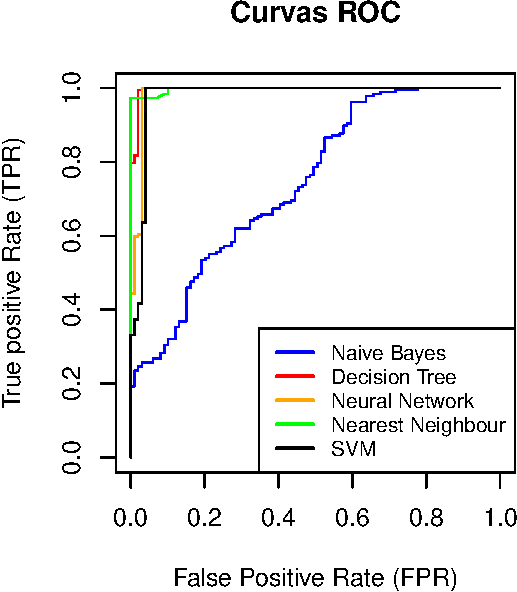
\includegraphics{R_2_files/figure-latex/unnamed-chunk-12-1.pdf}

\end{document}
